% !TEX root = poster.tex
\node [mybox,anchor=north west, font=\fontsize{\fntszL}{\fntszL}\selectfont]
at (\predPos) (boxPred){%
\begin{minipage}{\bxszB}

\medskip
\medskip
\medskip
 \medskip
\centerline{
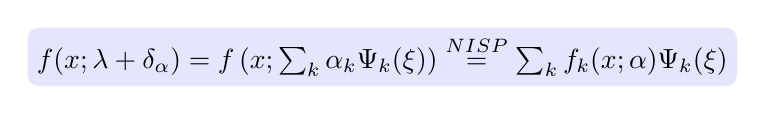
\begin{tikzpicture} \node [rounded corners,fill=blue!10] {
$f(x;\lambda+\delta_\alpha)=f\left(x;\sum_k \alpha_k \Psi_k(\xi)\right)\stackrel{NISP}{=}\sum_{k} f_{k}(x;\alpha) \Psi_k(\xi)$
};
\end{tikzpicture}
}
\medskip
\medskip
 \medskip

  \begin{itemize}
\item Non-intrusive spectral projection (NISP) employed for
  \begin{itemize}
\item Likelihood computation and posterior predictions
\item Easy access to first two moments:
\[
\mu(x;\alpha)=f_0(x;\alpha), \qquad\quad\sigma^2(x;\alpha)=\sum_{k>0} f^2_k(x;\alpha) ||\Psi_k||^2
\]
\end{itemize}
\vspace*{-0.7cm}
\item Predictive mean
\vspace*{-1.4cm}
\[
\qquad\quad\mathbb{E}[y(x)]=\mathbb{E}_\alpha[\mu(x;\alpha)]
\]
\item Decomposition of predictive variance
\[
\mathbb{V}[y(x)]=\underbrace{\mathbb{E}_{\alpha}[\sigma^2(x;\alpha)]}_{\textrm{Model error}}+\underbrace{\mathbb{V}_{\alpha}[\mu(x;\alpha)]+\sigma_d^2}_{\textrm{Poserior/Data error}}
\]
\end{itemize}


\centerline{
\includegraphics[width=0.94\textwidth]{merr/merr_workflow.png}
}

\end{minipage}
};
\node[fancytitle, right=10pt, font=\fontsize{\fntszL}{\fntszL}\selectfont]
at (boxPred.north west) {\bf Forward Prediction with Polynomial Chaos};
